
\chapter{Basics of Algorithm Complexity\label{chpt:computing-performance}}

Algorithm complexity is one of the crucial criteria to evaluate the theoretical
performance of the code, as defined below:

Let $f$ and $g$ be two functions defined over the natural numbers
$\mathbb{N}$. We write
\begin{equation}
f=O(g)
\end{equation}
if there is a strictly positive constant $c>0$ such that from a certain
number $n>n_{0}$ we always have $\left|f(n)\right|\leq c\left|g(n)\right|$.
The $O$ is also called the big-O notation \citep{Complexity}, or
order of growth. Figure \ref{fig:order-of-growth} shows the growth
tendency of some frequent functions. We can see:
\begin{equation}
O(1)>O(\log_{2}n)>O(n)>O(n\log_{2}n)>O(n^{2})>O(2^{n})>O(n!)
\end{equation}

\begin{figure}[h]
\begin{centering}
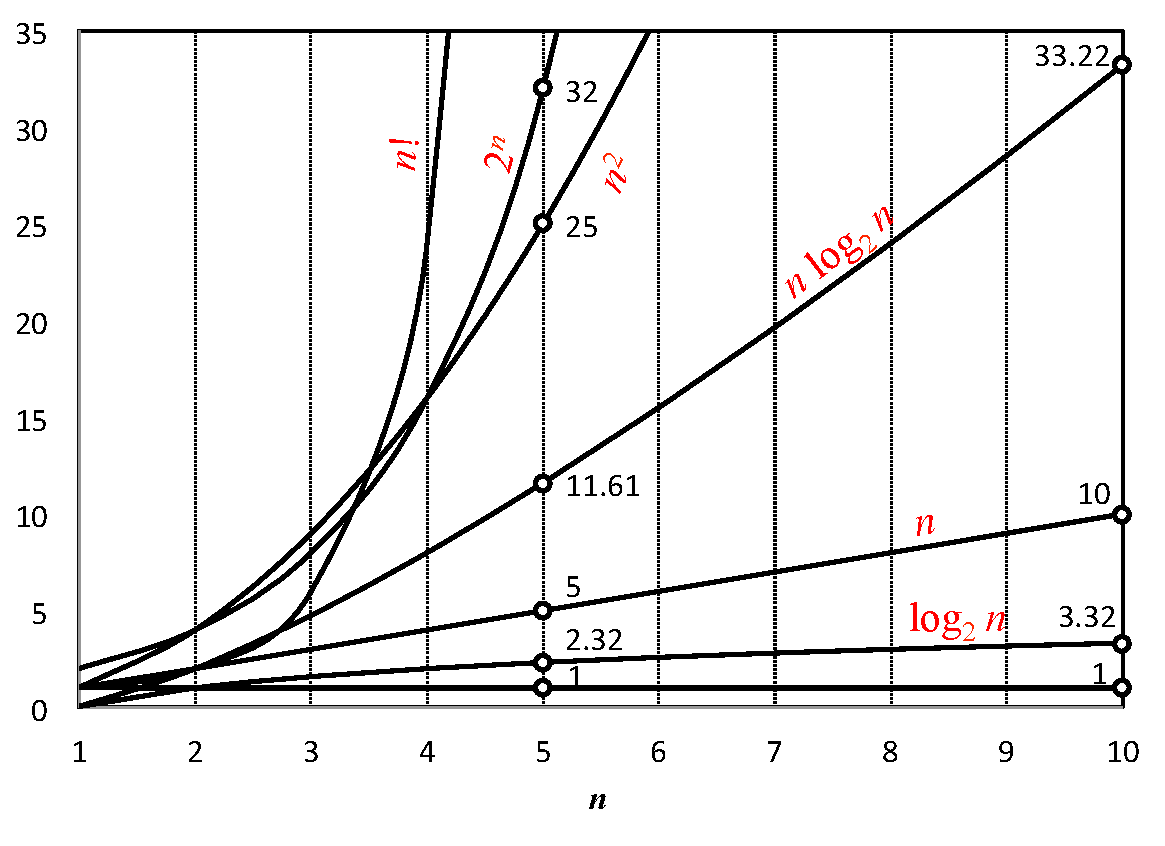
\includegraphics[width=0.75\textwidth]{_figure/orders-of-growth}
\par\end{centering}
\caption{Function growth\label{fig:order-of-growth}}
\end{figure}

In this thesis, the big-O notation is used to measure algorithm complexity.
Other notations can also be used for the same purpose, such as:
\begin{itemize}
\item $f=o(g)$ if $f(n)/g(n)\rightarrow0$, $n\rightarrow\infty$
\item The inverse of big-O notation $f=\Omega(g)$ if $g=O(f)$
\item The notation $f=\Theta(g)$ means that both $f=O(g)$ and $g=O(f)$
hold, and we can also say they are of the same order.
\end{itemize}
In code development we always search for algorithms with a lower algorithm
complexity. Ideally, the implementation of code matches the model
and has the same growth tendency as its complexity. But in the practical
case, overheads and memory delay can also limit the performance.
